%% Example data sheet
%% Feel free to modify and use this file for any purpose, under
%% either the LaTeX Project Public License or under public domain.

% Options here are passed to the article class.
% Most common options: 10pt, 11pt, 12pt
\documentclass[11pt]{datasheet}

% Input encoding and typographical rules for English language
\usepackage[utf8]{inputenc}
\usepackage[english]{babel}
\usepackage[english]{isodate}
\usepackage{pdfpages}

\usepackage{graphicx}

% tikz is used to draw images in this example, but you can
% also use \includegraphics{}.
\usepackage{tikz}
\usepackage{pgfplots}
\usepgfplotslibrary{groupplots}
\usepackage{circuitikz}
\usetikzlibrary{calc}

\usepackage{mhchem}

\usepackage{listings}
\lstset{
    basicstyle=\ttfamily\small,
    breaklines=true,
    columns=flexible,
    keywordstyle=\color{blue},
    stringstyle=\color{red},
    commentstyle=\color{green},
    showstringspaces=false,
    escapeinside={(*@}{@*)}
}

% These define global texts that are used in headers and titles.
\title{1S3P LTO Battery Pack with BMS}
\author{\textmu{}Art.cz}
\date{April 2025}
\revision{Document Revision 2}
\companylogo{logo.pdf}

\begin{document}
\maketitle

\section{Features}

\begin{itemize}
\item{Battery Chemistry: Lithium Titanate (LTO) for an extended lifespan and extreme }temperature resilience.
\item{Configuration: 1S3P (three LTO 18650 cells in parallel).}
\item{Nominal Voltage: 2.4 V}
\item{Voltage Range: 1.5 - 2.8 V}
\item{Capacity: 3.9 Ah (1300 mAh per cell)}
\item{BMS Features:}
    \begin{itemize}
    \item{Overvoltage and undervoltage protection}
    \item{Overcurrent protection}
    \item{I2C communication for real-time battery monitoring (voltage, current, power)}
    \item{User-upgradable firmware (UPDI programming interface)}
    \end{itemize}
\item{Fully open-source firmware, available on \href{https://github.com/slintak/lto-bms}{github.com} under the MIT license}
\end{itemize}

\section{Applications}

\begin{itemize}
\item{LoRa devices like Meshtastic, MeshCore, or Reticulum, \ldots}
\item{IoT and battery powered sensors}
\item{HAM radio setups}
\item{DIY outdoor and low-power electronics}
\end{itemize}

% Switch to next column
\vfill\break

\section{General Description}

This 1S3P Lithium Titanate (LTO) battery pack is designed for
low-power outdoor applications such as Meshtastic nodes, IoT,
HAM radio setups, and DIY electronics. It features an integrated
smart Battery Management System (BMS) with voltage, current, and
energy measurement, along with protection features including
under-voltage lockout (UVLO), over-voltage lockout (OVLO), and
overcurrent protection (OC). The battery pack communicates via
I\textsuperscript{2}C, allowing real-time monitoring of power
parameters.

This project is \textbf{partially open-source}, with public
schematics, 3D model in STEP format, 3D printable enclosure,
bill of materials (BOM), and
\href{https://github.com/slintak/lto-bms}{firmware}.

\begin{figure}[!ht]
\centering
\resizebox{0.45\textwidth}{!}{%
\begin{circuitikz}
\tikzstyle{every node}=[font=\tiny]
\node at (4,9.75) [circ] {};
\node at (5,9.75) [circ] {};
\node at (4,8.75) [circ] {};
\node at (5,8.75) [circ] {};
\draw (5,8.75) to[battery1] (5,9.75);
\draw (4,8.75) to[battery1] (4,9.75);
\draw (3,8.75) to[battery1] (3,9.75);
\draw (3,9.75) to[short] (5.75,9.75);
\draw (3,8.75) to[short] (5.75,8.75);
\draw  (5.75,10.25) rectangle  node {\LARGE BMS} (7.75,8.25);
\draw  (5.75,6.75) rectangle  node {\LARGE MCU} (7.75,5.5);
\draw [->] (6,6.75) -- (6,8.25)node[pos=0.5,fill=white]{SCL};
\draw [<->] (6.75,6.75) -- (6.75,8.25)node[pos=0.5, fill=white]{SDA};
\draw [short] (7.5,6.75) -- (7.5,8.25)node[pos=0.5,fill=white]{GND};
\draw (9.75,9.75) to[european resistor,l={ \normalsize $R_{load}$}] (9.75,8);
\draw [ dashed] (8,10.5) rectangle  (2.5,8);
\node [font=\normalsize] at (4.25,10.75) {LTO pack with BMS};
\draw (11.5,9.75) to[american voltage source,l={\normalsize Charger}] (11.5,8);
\draw (9.75,9.75) to[short] (7.75,9.75);
\draw (7.75,8.75) to[short] (8.5,8.75);
\draw (8.5,8.75) to (8.5,7.75) node[ground]{};
\draw (9.75,8) to (9.75,7.75) node[ground]{};

\draw [dashed] (9.75,9.75) -- (11.5,9.75);
\node at (9.75,9.75) [circ] {};
\draw (11.5,8) to (11.5,7.75) node[ground]{};
\end{circuitikz}
}%

\centerline{%
    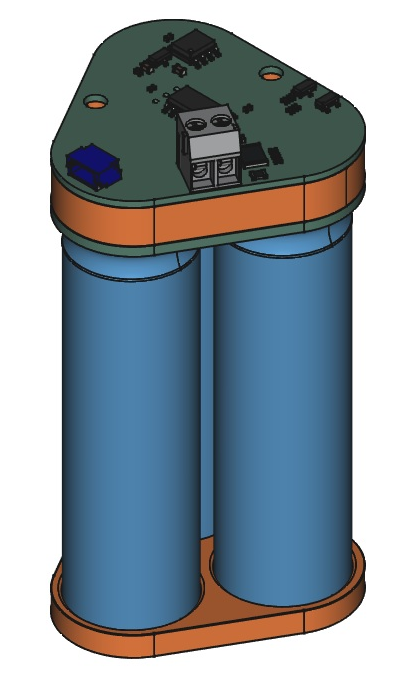
\includegraphics[width=0.2\textwidth]{../docs/LTO-BMS-revB-overview.png}
}
\caption{Block diagram (top) and a 3D render (bottom) of the product.}
\label{fig:block-diagram}
\end{figure}

% For wide tables, a single column layout is better. It can be switched
% page-by-page.
\onecolumn

\section{Absolute Maximum Ratings}

\begin{table}[ht]
\caption{Absolute Maximum Ratings of LTO Battery Pack}
\begin{tabularx}{\textwidth}{l | X }
    \thickhline
    \textbf{Parameter} & \textbf{Rating} \hspace{5cm} \\
    \hline
    Maximum Charging Voltage & 2.8 V \\
    Minimum Voltage & 1.5 V \\
    Maximum Charging Current & 1.0 A (0.25C)\\
    Maximum Discharging Current & 1.0 A (0.25C) \\
    Operating Temperature Range & -40\degree{}C to +60\degree{}C \\
    \thickhline
\end{tabularx}
\end{table}

\textbf{Note:} Stresses above those listed under Absolute Maximum Ratings can
cause permanent damage to the device. Charging and discharging currents are
limited by the electronics of the BMS, not by the LTO cells itself.
 
\section{Electrical Specifications}
All specifications are in $-40\degree C \leq T_A \leq 60\degree C$ unless otherwise noted.

\begin{table}[ht]
\begin{threeparttable}
\caption{LTO Battery Pack Electrical Specifications}
\begin{tabularx}{\textwidth}{l | c | c c c | c | X}
    \thickhline
    \textbf{Parameter} & \textbf{Symbol} & \textbf{Min.} & \textbf{Typ.} & \textbf{Max.} &
    \textbf{Unit} & \textbf{Note} \\
    \hline
    Nominal Capacity & $C_{nom}$ & & 3900 & & mAh & \\
    Capacity at -20\degree{}C & $C_{-20}$ & & $\geq 90\%$ of $C_{nom}$ & & mAh & \\
    Capacity at -40\degree{}C & $C_{-40}$ & & $\geq 50\%$ of $C_{nom}$ & & mAh & \\
    Cell Voltage & $V_{cell}$ & 1.5 & 2.4 & 2.8 & V & \tnote{1} \\
    Internal Impedance & $R_{int}$ & & & 18 & m$\Omega$ & \tnote{2} \\
    Charging Current & $I_{charge}$ & & 1.0 & 2.0 & A & \tnote{3} \tnote{4} \\
    Discharging Current & $I_{discharge}$ & & 1.0 & 2.0 & A & \tnote{3} \tnote{4} \\
    Operating Temperature Range & $T_{oper}$ & -40 & & 60 & \degree{}C & \\
    Weight & $W_{total}$ & & 133 & & g & \\
    Cycle Life ($\geq$ 80\% of nominal capacity) & $N_{cycles}$ & 5000 & & & cycles & \\
    \thickhline
\end{tabularx}
\begin{tablenotes}
\item[1]{Typical $V_{cell}$ value is nominal (average) voltage of one LTO cell.}
\item[2]{Internal impedance of one LTO cell, not the whole battery pack.}
\item[3]{Typical currents can be continuous and are limited by the BMS, not the LTO cells itself.}
\item[4]{Maximum currents recommended for $t_{max} = 120 s$.}
\end{tablenotes}
\end{threeparttable}
\end{table}

\clearpage
\section{Detailed Description}

Lithium Titanate Oxide (LTO) batteries are a distinct category within the
rechargeable lithium-based battery family, utilizing lithium titanate
(\ce{Li4Ti5O12}) as the anode material. This composition gives LTO cells
unique characteristics that differentiate them from other lithium-ion
chemistries, such as Lithium-Ion (Li-Ion), Lithium Polymer (Li-Po), and
Lithium Iron Phosphate (\ce{LiFePO4}, or LFP) batteries.

LTO batteries present a compelling option for applications requiring long cycle
life, operation in extreme temperatures, and rapid charging. However, their
lower energy density and higher cost may limit their suitability for
applications where space and budget are primary concerns.

An LTO cell typically operates within the voltage ranges shown in Table~\ref
{tab:lto-comparison}. These voltage ranges are lower compared to other
lithium-based batteries, necessitating appropriate system design considerations
when integrating LTO cells into the intended application. They are not and
cannot be a drop-in replacement for Li-Ion, Li-Po and other types of batteries
and cannot be charged by their charging ICs.

With the parameters in Table~\ref{tab:lto-comparison}, one can see that LTO
batteries are a great fit for battery-powered, low-power devices installed
outdoors year-round.

\begin{table}[ht]
\centering
\caption{Comparison of LTO, Li-Ion/Li-Po, and \ce{LiFePO4} Batteries}
\label{tab:lto-comparison}
\begin{tabularx}{\textwidth}{l | c | c | c | c}
\thickhline
\textbf{Parameter} & \textbf{Unit} & \textbf{LTO} & \textbf{Li-Ion/Li-Po} & \textbf{\ce{LiFePO4}} \\
\hline
Nominal Voltage & V & 2.3–2.4 & 3.6–3.7 & 3.2–3.3 \\
Maximum Voltage & V & 2.8–2.9 & 4.2–4.4 & 3.65 \\
Minimum Voltage & V & 1.5–1.6 & 2.5–3.0 & 2.5 \\
Energy Density & Wh/kg & 70–110 & 150–250 & 90–160 \\
Cycle Life & cycles & 4000–7000 & 500–1,500 & 2,000–5,000 \\
Charge Rate & C & 5–10 & 1–2 & 1–2 \\
Discharge Rate & C & 10–20 & 1–10 & 10–25 \\
Discharging Temp. Range & \degree{}C & -40 to 60 & -20 to 60 & -20 to 60 \\
Charging Temp. Range & \degree{}C & -10 to 55 & 0 to 45 & 0 to 45 \\
Safety & -- & Very High & Medium & High \\
\thickhline
\end{tabularx}
\end{table}

\subsection{Advantages of LTO Cells}

\begin{itemize}
\item \textbf{Extended Cycle Life:} They can endure a significantly higher number of charge-discharge cycles, often exceeding 4000 cycles, which is substantially more than typical Li-Ion or \ce{LiFePO4} batteries.
\item \textbf{Enhanced Safety:} The structural stability of LTO reduces risks associated with thermal runaway, making them safer under various operating conditions.
\item \textbf{Wide Operating Temperature Range:} LTO batteries perform reliably in a broad temperature spectrum, including sub-zero conditions, making them suitable for extreme environments.
\item \textbf{Rapid Charging:} LTO cells support high charge and discharge rates, allowing for quick charging times. This is less important for IoT and low-power devices which this LTO battery pack with BMS is designed for.
\end{itemize}

\subsection{Disadvantages of LTO Cells}

\begin{itemize}
\item \textbf{Lower Energy Density:} They typically offer energy densities between 30–110 Wh/kg, which is lower than that of Li-Ion and LiFePO$_4$ batteries.
\item \textbf{Higher Cost:} The advanced materials and manufacturing processes contribute to a higher price point compared to other lithium-ion batteries.
\end{itemize}

\section{Protection Features}

The Battery Management System (BMS) includes essential protection mechanisms to
ensure safe and reliable operation of Lithium Titanate Oxide (LTO) cells. These
mechanisms protect against overvoltage (OVLO), undervoltage (UVLO), and
overcurrent (OC) conditions. All protection thresholds are fully configurable
by writing new values into the EEPROM memory of the BMS's main microcontroller,
an \texttt{ATtiny824}.

\textbf{Overvoltage protection} ensures that the cell voltage does not exceed a
 safe upper limit. When the measured voltage on the LTO cells rises above the
 configured cutoff threshold (\texttt{ovlo\_cutoff}), the BMS disconnects the
 charging path. Charging is only re-enabled once the voltage falls below the
 defined release level (\texttt{ovlo\_release}). This protects the cell from
 overcharging, which could otherwise reduce its lifespan or cause safety
 hazards.

To prevent \textbf{over-discharge} and possible damage to the LTO cells, the BMS
continuously monitors the voltage level of the cells and disconnects the load
if the voltage drops below the cutoff threshold (\texttt{uvlo\_cutoff}). The
load remains disconnected until the voltage recovers above the release
threshold (\texttt{uvlo\_release}). This functionality helps preserve battery
health and avoids deep discharge scenarios.

The BMS also includes \textbf{overcurrent protection} on the output. If the
current exceeds the \texttt{max\_current} setting (in mA), the output is
disabled. The duration of the overcurrent condition is monitored, and if it
persists longer than the configured timeout (\texttt{oclo\_timeout}, in
milliseconds), the output is turned off to prevent overheating or damage to
connected circuitry.

All protection parameters can be configured by the user via a Python tool
included in the firmware repository. This tool allows writing new settings into
the EEPROM of the \texttt{ATtiny824} via UPDI programming interface, enabling
customization for different applications, usage scenarios, or safety
requirements. Their default parameters are in Table~\ref
{tab:bms-protection-config}.

\begin{table}[ht]
\centering
\caption{Default BMS EEPROM Configuration}
\label{tab:bms-protection-config}
\begin{tabularx}{\textwidth}{>{\raggedright\arraybackslash}l 
                                  >{\raggedright\arraybackslash}X 
                                  >{\raggedleft\arraybackslash}l}
\thickhline
\textbf{Parameter} & \textbf{Description} & \textbf{Default Value} \\
\hline
\texttt{serial\_number} & Device serial number & 0 \\
\texttt{temp\_offset}   & Temperature sensor offset (\degree{}C) & 0 \\
\texttt{ovlo\_cutoff}   & Overvoltage cutoff threshold (mV) & 2800 \\
\texttt{ovlo\_release}  & Overvoltage release threshold (mV) & 2700 \\
\texttt{uvlo\_release}  & Undervoltage release threshold (mV) & 1800 \\
\texttt{uvlo\_cutoff}   & Undervoltage cutoff threshold (mV) & 1700 \\
\texttt{max\_current}   & Maximum output current (mA) & 1000 \\
\texttt{oclo\_timeout}  & Overcurrent shutdown delay (s) & 10 \\
\thickhline
\end{tabularx}
\end{table}

\section{Charging}

The charging process of the Lithium Titanate Oxide (LTO) cells is
straightforward, thanks to the Battery Management System (BMS), which
implements all necessary safety features. Charging can be done simply by
connecting a constant voltage source to the load side of the BMS. The
recommended constant voltage range is 2.7--2.8~V, ensuring the voltage does not
exceed the maximum cell voltage.

The typical charging process is shown in Figure~\ref{fig:lto-charging}, where
the constant voltage was set to 2.85~V (slightly above the recommended range to
show \texttt{OVLO} state in the graph), and the battery's initial state
was \texttt{UVLO} (Under-Voltage Lockout), i.e., fully discharged. Charging is
considered complete when the cell voltage if above 1.7~V or when BMS activates
the \texttt{OVLO} (Over-Voltage Lockout), which indicates the battery is fully
charged.

As seen in the Figure~\ref{fig:lto-charging}, the cell voltage slowly increases
from 2.36~V(the voltage immediately after connecting the constant voltage
source to the load side) up to 2.8~V. At this point, the BMS disconnects the
cells from the load and activates \texttt{OVLO}.

The charging current is not limited by the constant voltage source, and thus it
starts at over 1.5 A, gradually decreasing to 0.173 A just before the battery
is fully charged. The entire 3900 mAh capacity is charged in less than 300
minutes (5 hours).

This charging procedure is simple and effective, as the BMS handles all the
necessary protections for the cells. A simple Low Dropout Regulator (LDO) or a
DC/DC converter can be used to provide the constant voltage for the battery,
making it easy and cost-effective to integrate into the user's project.

However, this method is still not ideal. Charging the battery with high current
when deeply discharged can lead to slight degradation of the cells, shortening
their lifespan and reducing the number of available charge cycles.

A slightly more advanced version of this setup uses an LDO or DC/DC converter
with a current limiting circuit. In this case, the output voltage is still set
to 2.7--2.8~V, but the current is limited, for example, to 0.5~A. This limits
the charging current at the beginning of the process, when the battery is
deeply discharged and most sensitive to high currents. This approach offers
better cell protection while maintaining simplicity and low cost.

The best, although more complex and costly, solution is to use a \textit
{Constant Current / Constant Voltage} (CC/CV) charger specifically designed for
LTO batteries, such as the CN3795 IC.


\begin{figure}[ht]
    \centering
    \caption{Charging of deeply discharged LTO battery with BMS by a constant voltage.}
    \label{fig:lto-charging}
    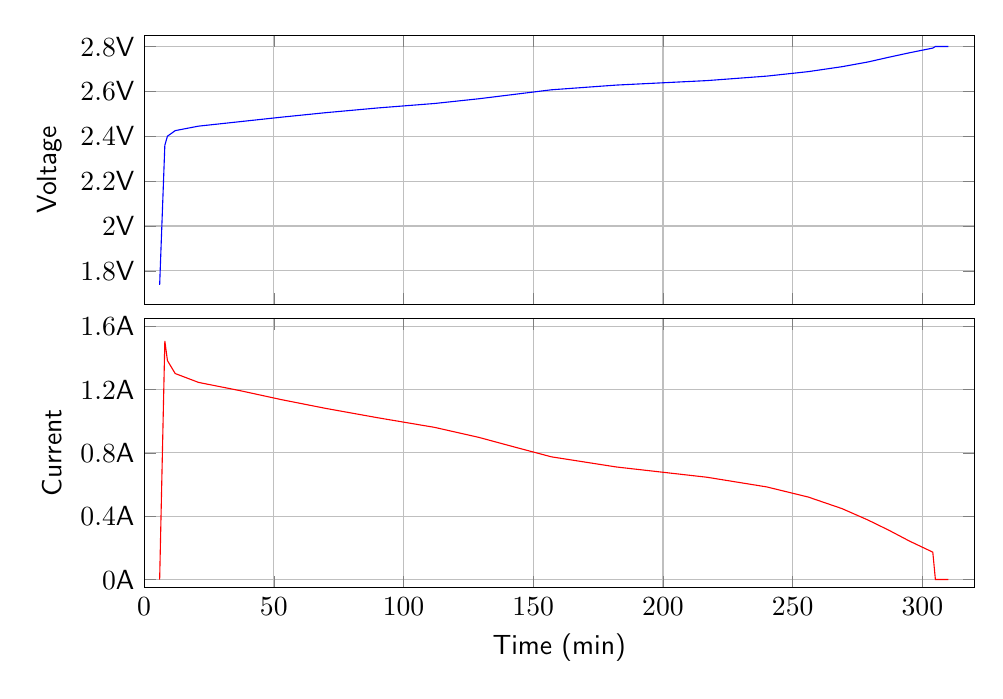
\begin{tikzpicture}
        \sffamily
        \begin{groupplot}[
            group style={
                % set how the plots should be organized
                group size=1 by 2,
                % only show ticklabels and axis labels on the bottom
                x descriptions at=edge bottom,
                % set the `vertical sep' to zero
                vertical sep=5pt,
            },
            width=\textwidth,
            height=5cm,
        ]
        % Plot for voltage (top plot)
        \nextgroupplot[
            ylabel={Voltage},
            ymode=normal,
            ytick distance=0.2,
            xmin=0, xmax=320,
            ymin=1.7, ymax=2.8,
            enlarge y limits={abs=0.05},
            xtick distance=50,
            yticklabel={\pgfmathprintnumber{\tick}V},
            xmajorgrids, ymajorgrids
        ]
        \addplot [blue] coordinates {
            (6,1.737)
            (8,2.36)
            (9,2.4)
            (12,2.425)
            (21,2.445)
            (37,2.465)
            (53,2.485)
            (70,2.505)
            (90,2.526)
            (112,2.546)
            (129,2.567)
            (143,2.587)
            (157,2.607)
            (182,2.628)
            (217,2.648)
            (240,2.668)
            (256,2.688)
            (269,2.71)
            (279,2.731)
            (287,2.752)
            (295,2.772)
            (304,2.793)
            (305,2.800)
            (310,2.800)
        };

        % Plot for current (bottom plot)
        \nextgroupplot[
            ylabel={Current},
            ymode=normal,
            xlabel={Time (min)},
            ytick distance=0.4,
            xmin=0, xmax=320,
            ymin=0, ymax=1.6,
            enlarge y limits={abs=0.05},
            xtick distance=50,
            yticklabel={\pgfmathprintnumber{\tick}A},
            xmajorgrids, ymajorgrids
        ]
        \addplot [red] coordinates {
            (6,0)
            (8,1.507)
            (9,1.383)
            (12,1.301)
            (21,1.245)
            (37,1.193)
            (53,1.136)
            (70,1.081)
            (90,1.022)
            (112,0.961)
            (129,0.898)
            (143,0.836)
            (157,0.775)
            (182,0.711)
            (217,0.646)
            (240,0.585)
            (256,0.521)
            (269,0.448)
            (279,0.376)
            (287,0.312)
            (295,0.243)
            (304,0.173)
            (305,0)
            (310,0)
        };
        \end{groupplot}
    \end{tikzpicture}
\end{figure}

\section{UART Interface}

The BMS outputs a detailed log containing the internal state and measurements of
the system every minute (this interval can be configured at compile time in the
firmware). This log is transmitted via the UART's \texttt{TXD} pin and uses the
\textbf{InfluxDB Line Protocol}, making it convenient to capture and store the
 data in an InfluxDB instance.

An example of this log is shown in Listing~\ref{lst:uart-output}, while the meaning
of each field is summarized in Table~\ref{tab:uart-fields}, and the possible
values of the \texttt{state} field are listed in Table~\ref{tab:bms-states}.

The UART interface provides a single \texttt{TXD} (transmit) signal and operates
at a baud rate of 9600. Please note that the BMS does not support receiving
data via \texttt{RXD}; it only transmits log data. The format of the
transmitted log is demonstrated in Listing~\ref{lst:uart-output}.

\begin{figure}[!h]
    \centering
    \begin{lstlisting}[caption={UART Output Example}, label={lst:uart-output}, linewidth=0.81\textwidth]
    lto-bms,id=0006
      uptime=3261420i,v_batt=2768i,v_load=2813i,current=-260i,E_dis=8163i,
      E_chg=15176i,charge=-2530i,temp=296i,gain=8i,state="BMS_STATE_CHARGING"
    \end{lstlisting}
\end{figure}



\begin{table}[!ht]
\centering
\caption{UART Log Fields Description}
\begin{tabularx}{\textwidth}{l|l|X}
\thickhline
\textbf{Field} & \textbf{Unit} & \textbf{Description} \\
\hline
\texttt{uptime}     & s        & Number of seconds since the last restart. \\
\texttt{v\_batt}    & mV       & Battery voltage. \\
\texttt{v\_load}    & mV       & Voltage present at the load side of the BMS. \\
\texttt{current}    & mA       & Current through the shunt resistor. Negative values indicate charging. \\
\texttt{E\_dis}     & Wh       & Energy discharged from the battery. \\
\texttt{E\_chg}     & Wh       & Energy charged into the battery. \\
\texttt{charge}     & Ah       & Total amount of charge in the battery. \\
\texttt{temp}       & K        & Internal temperature sensor reading. \\
\texttt{gain}       & –        & ADC gain setting for current measurement. \\
\texttt{state}      & –        & Internal BMS state. See Table~\ref{tab:bms-states}. \\
\thickhline
\end{tabularx}
\label{tab:uart-fields}
\end{table}

\begin{table}[!ht]
\centering
\caption{Possible BMS States in the UART Log}
\begin{tabularx}{\textwidth}{l|X}
\thickhline
\textbf{State} & \textbf{Description} \\
\hline
\texttt{BMS\_STATE\_INVALID}      & Invalid state. \\
\texttt{BMS\_STATE\_UVLO}         & Under-voltage lockout. \\
\texttt{BMS\_STATE\_OVLO}         & Over-voltage lockout. \\
\texttt{BMS\_STATE\_OVLO\_ACTIVE} & Over-voltage lockout active. \\
\texttt{BMS\_STATE\_OCLO}         & Over-current lockout. \\
\texttt{BMS\_STATE\_CHARGING}     & Charging. \\
\texttt{BMS\_STATE\_DISCHARGING}  & Discharging. \\
\texttt{BMS\_STATE\_IDLE}         & Idle. \\
\texttt{BMS\_STATE\_ERR}          & Error state. \\
\thickhline
\end{tabularx}
\label{tab:bms-states}
\end{table}

\section{I\textsuperscript{2}C Interface}

The battery management system (BMS) features an I\textsuperscript{2}C
interface for communication with external devices such as the Meshtastic
firmware. This allows the user to read power, current, and voltage
information from the battery without requiring any firmware modification
on the Meshtastic side, as it already supports the INA260.

This interface supports standard modes of communication and adheres
to the INA260 register structure, ensuring compatibility with
Meshtastic firmware and ease of integration into existing systems.

The I\textsuperscript{2}C interface of the BMS mimics the INA260's
register set. The communication protocol and register mapping are
identical to that of the INA260. Table~\ref{tab:register-set}
is a summary of the available registers.

\begin{table}[!ht]
\begin{threeparttable}
\caption{Register Set Summary}
\label{tab:register-set}
\begin{tabularx}{\textwidth}{ c | c | X | c | c | c }
    \thickhline
    \textbf{Address} & \textbf{Register Name} & \multicolumn{1}{c |}{\textbf{Function}} & \multicolumn{2}{c|}{\textbf{Power-on reset}} & \textbf{Type}\tnote{1} \\
    \cline{4-5}
    & & & Binary & Hex & \\
    \hline
    0x00 & Configuration Register\tnote{2} & All-register reset, shunt voltage and bus voltage ADC conversion times and averaging, operating mode. & 01100001 00100111 & 0x6127 & $R/\overline{W}$ \\ 
    0x01 & Current Register & Contains the value of the current flowing through the shunt resistor. & 00000000 00000000 & 0x0000 & R \\
    0x02 & Voltage Register & Voltage of the battery cell. & 00000000 00000000 & 0x0000 & R \\
    0x03 & Power Register & Contains the value of the calculated power being delivered from the battery.  & 00000000 00000000 & 0x0000 & R \\
    0xFE & Manufacturer ID Register\tnote{3} & Contains unique manufacturer identification number. & 01010100 01001001 & 0x5449 & R \\
    0xFF & Die ID Register\tnote{3} & Contains unique die identification number. & 00100010 01110000 & 0x2270 & R \\
    \thickhline
\end{tabularx}
\begin{tablenotes}
\item[1]{Type: \textbf{R} = Read-only, $\mathbf{R/\overline{W}}$ = Read/Write.}
\item[2]{This register is present only for the compatibility with INA260 and is ignored by the current firmware.}
\item[3]{These registers and their values are the same as those of the INA260 to mimic the interface.}
\end{tablenotes}
\end{threeparttable}
\end{table}

\section{Calculating Returned Values}

The least significant bit (LSB) sizes for the \textit{Bus Voltage Register},
\textit{Current Register}, and \textit{Power Register} are fixed, as shown in
Table~\ref{tab:register_calculations}. To calculate any of the values
for current, voltage, or power, take the integer value returned by
the device and multiply that value by the corresponding LSB size.

For example, the LSB for the bus voltage is 1.25 mV/bit. If the device
returns an integer value of 9584 (0x2570), the value of the battery voltage
is calculated as:

\[
V_{battery} = 1.25\ \text{mV} \times 9584 = 11.98\ \text{V}.
\]

Since the system supports current measurements in both directions,
the returned value for negative currents (battery charging, current
flowing into the LTO battery) is represented in two's complement
format. The returned power values will always be positive, even
when the current is negative.

\begin{table}[ht]
\centering
\caption{Calculating Current, Voltage, and Power}
\begin{tabularx}{\textwidth}{c|c|c|c|c|c}
\thickhline
\textbf{Register Name} & \textbf{Address} & \textbf{LSB} & \multicolumn{2}{c|}{\textbf{Example}} & \textbf{Note} \\
\cline{4-5}
& & & \textbf{Integer Value} & \textbf{Result} & \\ 
\hline
Current Register & 0x01 & 1.25 mA & 0x02F8 & 0.95 A & \\
Voltage Register & 0x02 & 1.25 mV & 0x0898 & 2.75 V & \\
Power Register & 0x03 & 1.25 mW & 0x082A & 2.6125 W & \\
\thickhline
\end{tabularx}
\label{tab:register_calculations}
\end{table}

This table summarizes the calculation of the returned values for
current, voltage, and power. When working with the returned data,
it is important to multiply the raw register value by the
appropriate LSB size to obtain the correct measurement in either
volts, milliamps, or milliwatts.

\section{Self-Consumption}

The Figure~\ref{fig:self-consumption} shows the approximate power consumption of
the BMS circuit at different battery voltages. These measurements
are indicative and will likely change as the firmware is further
optimized. There are still many areas in the code that can be optimized.

\begin{figure}[ht]
    \centering
    \begin{minipage}{0.48\textwidth}
        \centering
        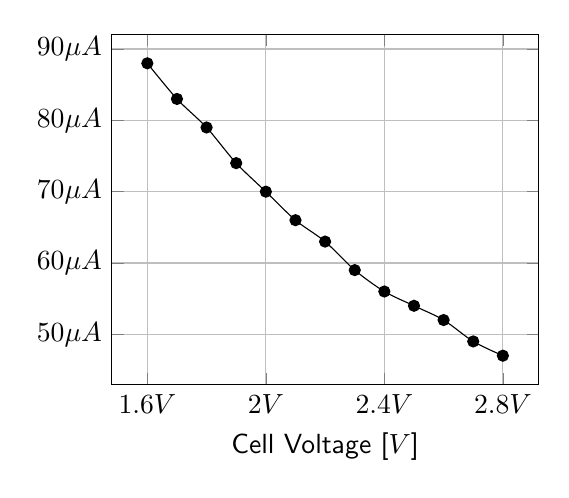
\begin{tikzpicture}
            \sffamily
            \begin{axis}[
                width=7cm,
                xlabel={Cell Voltage [$V$]},
                xtick distance=0.4,
                ytick distance=10,
                xticklabel={\pgfmathprintnumber{\tick}$V$},
                yticklabel={\pgfmathprintnumber{\tick}$\mu{}A$},
                xmajorgrids, ymajorgrids]
            \addplot[smooth,mark=*] plot coordinates {
                (1.60, 88)
                (1.70, 83)
                (1.80, 79)
                (1.90, 74)
                (2.00, 70)
                (2.10, 66)
                (2.20, 63)
                (2.30, 59)
                (2.40, 56)
                (2.50, 54)
                (2.60, 52)
                (2.70, 49)
                (2.80, 47)
            };
            \end{axis}
        \end{tikzpicture}
        \caption{Average self-consumption vs. battery voltage}
        \label{fig:self-consumption}
    \end{minipage}%
    \hfill
    \begin{minipage}{0.48\textwidth}
        \centering
        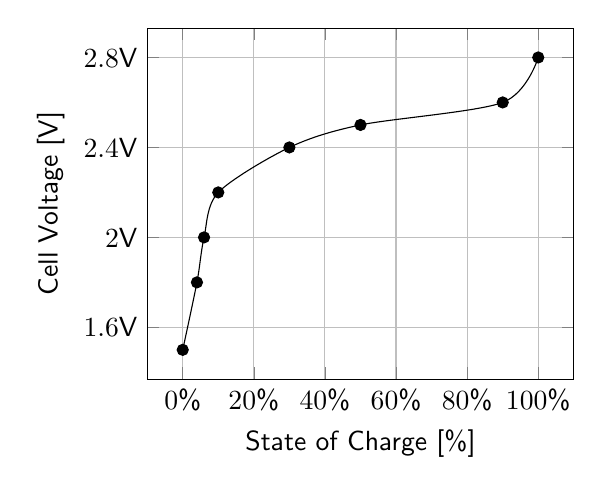
\begin{tikzpicture}
            \sffamily
            \begin{axis}[
                width=7cm,
                ylabel={Cell Voltage [V]},
                xlabel={State of Charge [\%]},
                xtick distance=20,
                ytick distance=0.4,
                xticklabel={\pgfmathprintnumber{\tick}\%},
                yticklabel={\pgfmathprintnumber{\tick}V},
                xmajorgrids, ymajorgrids]
            \addplot[smooth,mark=*] plot coordinates {
                (100, 2.8)
                (90, 2.6)
                (50, 2.5)
                (30, 2.4)
                (10, 2.2)
                (6, 2.0)
                (4, 1.8)
                (0, 1.5)
            };
            \end{axis}
        \end{tikzpicture}
        \caption{Typical LTO cell voltage vs. state of charge for a small discharge currents ($< 1C$).}
        \label{fig:lto-voltage}
    \end{minipage}
\end{figure}

Based on a typical cell voltage (see Figure~\ref{fig:lto-voltage}), we know that
the LTO battery maintains a voltage of around 2.45 V during low discharge
currents, and this voltage is sustained for most of the discharge cycle. The
voltage starts to drop significantly only when the battery is nearly fully
discharged. Therefore, we can estimate the average power consumption of the BMS
circuit to be 67.45 \textmu{}Ah. If a single 1300 mAh cell is connected to the
BMS without load, it will discharge in approximately 19,000 hours, or roughly 2
years.

\clearpage
\section{Schematics}

\begin{figure}[!ht]
    \centering
    \rotatebox{90}{%
        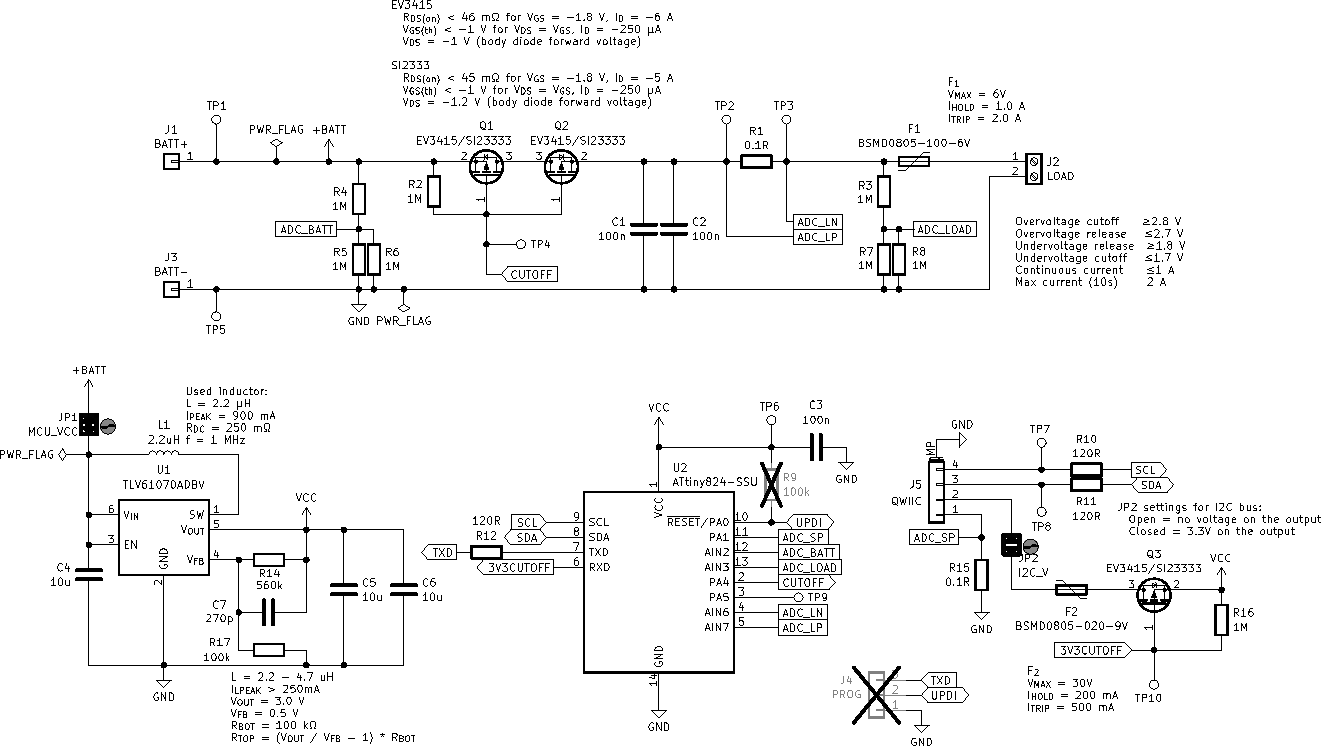
\includegraphics[width=1.2\textwidth]{../docs/LTO-BMS-revB-schematic-noborder.pdf}
    }
    \caption{Schematics of the battery management system (BMS) used in the 1S3P LTO battery pack with BMS.}
\end{figure}

\clearpage
\section{Mechanical Dimensions}

\begin{figure}[!ht]
    \centerline{%
        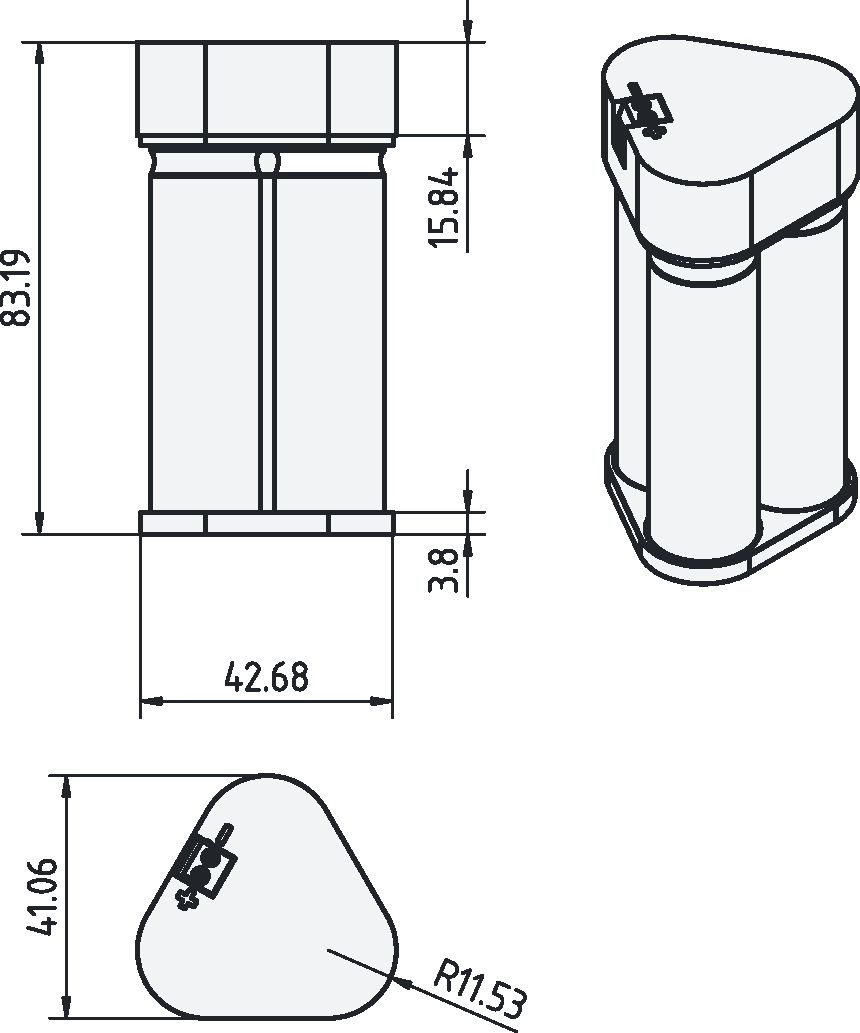
\includegraphics[width=0.8\textwidth]{../docs/LTO-BMS-revB-dimensions.pdf}
    }
    \caption{Mechanical dimenstions of the 1S3P LTO battery pack (using 3 $\times$ 18650 cells) with the BMS and 3D printed enclosures. Dimensions in mm.}
\end{figure}

\end{document}
